\documentclass{beamer}
\setbeamertemplate{footline}[frame number]
%\usepackage{beamerthemeBerkeley}
\usetheme{Montpellier}
%\usetheme{Warsaw}
%\usetheme{Boadilla}
\usepackage[english]{babel}
\usepackage{graphicx}
%\usepackage{ams}
%\usepackage{blue}
\usepackage{amsmath} 

\newcommand{\myp}{\ensuremath{\mathbb{P}}}
\newcommand{\mye}{\ensuremath{\mathbb{E}}}
\newcommand{\myvar}{\mathbf{Var}}
\newcommand{\mycov}{\mathbf{Cov}}
\newcommand{\myind}{\ensuremath{\mathbbm{1}}}

\newcommand{\mI}{\ensuremath{\pmb{\mathsf{I}}}}
\newcommand{\mL}{\ensuremath{\pmb{\mathsf{L}}}}
\newcommand{\mQ}{\ensuremath{\pmb{\mathsf{Q}}}}
\newcommand{\mV}{\ensuremath{\pmb{\mathsf{V}}}}
\newcommand{\mW}{\ensuremath{\pmb{\mathsf{W}}}}
\newcommand{\mX}{\ensuremath{\pmb{\mathsf{X}}}}
\newcommand{\mZ}{\ensuremath{\pmb{\mathsf{Z}}}}

\newcommand{\ba}{\mathbf{a}}
\newcommand{\bd}{\mathbf{d}}
\newcommand{\bg}{\mathbf{g}}
\newcommand{\bV}{\mathbf{V}}
\newcommand{\bX}{\mathbf{X}}
\newcommand{\bY}{\mathbf{Y}}
\newcommand{\bZ}{\mathbf{Z}}

\newcommand{\bzero}{\mathbf{0}}

\newcommand{\balpha}{\mbox{\boldmath$\alpha$}}
\newcommand{\bbeta}{\mbox{\boldmath$\beta$}}
\newcommand{\bepsilon}{\mbox{\boldmath$\epsilon$}}
\newcommand{\bgamma}{\mbox{\boldmath$\gamma$}}
\newcommand{\bDelta}{\mbox{\boldmath$\Delta$}}
\newcommand{\bPhi}{\mbox{\boldmath$\Phi$}}
\newcommand{\bPsi}{\mbox{\boldmath$\Psi$}}
\newcommand{\bSigma}{\mbox{\boldmath$\Sigma$}}
\newcommand{\bmu}{\mbox{\boldmath$\mu$}}



\title{Lecture 2: Introduction to the PLINK Software for GWAS \& Population Structure Inference}

\author{Instructors: Joelle Mbatchou and Loic Yengo} 


\date{}


\begin{document}
	
	
	
	\begin{frame}
		\titlepage
		\vspace{-2cm}
		\begin{center}
			
			{ \Large Summer Institute in Statistical Genetics 2022\\}
		

\end{center}
\end{frame}


\section{PLINK Software}
	
\begin{frame}
\frametitle{\bf PLINK Overview}
\begin{itemize}
\item PLINK is a free, open-source whole genome association analysis toolset, designed to perform a range of basic, large-scale analyses in a computationally efficient manner: \\
\vspace{.5em}
{\color{red}
\url{https://www.cog-genomics.org/plink/1.9/}
\url{https://www.cog-genomics.org/plink/2.0/}
}
\vspace{.5em}

\item PLINK has numerous useful features for managing and analyzing genetic data
\end{itemize}
\end{frame}

  \begin{frame}
	\frametitle{\bf PLINK Overview}
	\begin{itemize}
\item Data management
\begin{itemize}
	\item Read data in a variety of formats (BED, PGEN, BGEN, VCF,...)
	\item Convert between different formats
	\item Recode and reorder files
	\item Merge multiple genetic files
	\item Extracts subsets (SNPs or individuals)
\end{itemize}
	\end{itemize}
\end{frame}


  \begin{frame}
	\frametitle{\bf PLINK Overview}
	\begin{itemize}
\item Summary statistics for quality control
\begin{itemize}
	\item Allele \& genotypes counts/frequencies
	\item Missing genotype rates
	\item Mendel error rate
	\item HWE tests
	\item Sample  variant counts
	\item Inbreeding, IBS and IBD statistics for individuals and pairs of individuals
\end{itemize}
	\end{itemize}
\end{frame}


\begin{frame}
\frametitle{\bf PLINK Overview}
\begin{itemize}
\item Basic association testing
\begin{itemize}
		\item Standard allelic test \& Fisher's exact test for case-control data
	\item Linear and logistic regression
		\item Dominant/recessive and general models
		    \item Family-based association tests (e.g. TDT)
	\item Association conditional on one or more SNPs
	\end{itemize}

\end{itemize}
\end{frame}



\begin{frame}
\frametitle{\bf PLINK Overview}
\begin{itemize}
\item  Gene-based tests of association
\item Screen for epistasis
\item Gene-environment interaction with continuous and dichotomous environments
\item Meta-analysis
\begin{itemize}
    \item Automatically combine several generically-formatted summary files, for millions of SNPs
\end{itemize}
\end{itemize}
\end{frame}


\begin{frame}
\frametitle{\bf Input Files}
\begin{itemize}
\item PLINK BED: Genotype data is a compressed binary file (0/1)
\begin{itemize}
\item Fam File (.fam)  contains sample information
\item Bim file (.bim) contains variant information
\item Bed file (.bed) contains the genotype data
\end{itemize}
\end{itemize}
\end{frame}


\begin{frame}[fragile]
\frametitle{\bf Data Management}
\begin{itemize}
\item Inclusion/Exclusion criteria options
\begin{itemize}
\item   \begin{verbatim} --keep msamples.txt, --remove msamples.txt  \end{verbatim}
\item \begin{verbatim} --extract mysnps.txt, --exclude mysnps.txt \end{verbatim}
\item \begin{verbatim}  --chr 2,6 --from rs273744 --to rs89883 \end{verbatim}
\end{itemize}
\item  Other data management options
\begin{itemize}
\item \begin{verbatim}  --make-bed, --export, --pmerge \end{verbatim}
\end{itemize}
\item Using files with phenotypes/covariates
\begin{itemize}
\item  \begin{verbatim} --pheno, --covar \end{verbatim}
\end{itemize}
\end{itemize}
\end{frame}


\begin{frame}[fragile]
\frametitle{\bf Quality Control (QC)}
\begin{itemize}
\item Summary statistics options:
\begin{itemize}
\item  minor allele frequency (MAF): \verb+--freq +
\item  genotype counts: \verb+--geno-counts +
\item  SNP \&  individual missing rate:  \verb+--missing +
\item  Hardy-Weinberg:  \verb+--hardy +
\end{itemize}
\item Inclusion/Exclusion filters
\begin{itemize}
\item MAF:   \verb+--maf , --max-maf+
\item minor allele count (MAC):   \verb+--mac,--max-mac+
\item  SNP missing rate: \verb+--geno +
\item Individual missing rate:  \verb+--mind +
\item  Hardy-Weinberg:   \verb+--hwe +
\end{itemize}
\end{itemize}
\end{frame}



\begin{frame}[fragile]
\frametitle{\bf Association Analysis with PLINK}
With PLINK
\begin{itemize}
\item Association testing: \verb+--assoc, --linear, --logistic+
\item Conditional analysis: \verb+--condition-list+
\item GxE interaction: \verb+--gxe +
\end{itemize}
\vspace{1em}
With PLINK2
\begin{itemize}
	\item Association testing: \verb+--glm+
	\item Conditional analysis: \verb+--condition-list+
	\item GxE interaction: \verb+ --glm interaction +
\end{itemize}
\end{frame}




\begin{frame}[fragile]
\frametitle{\bf GWAS of Transferrin}
\begin{itemize}
\item PLINK input files:
\begin{itemize}
\item \verb+ Transferrin_height.bed+
\item \verb+ Transferrin_height.fam+
\item \verb+ Transferrin_height.bim+
\end{itemize}
\item Phenotype file:
\begin{itemize}
	\item \verb+ Transferrin_pheno.txt+
\end{itemize}
\item HELP: check the PLINK website documentation (very useful!)

\vspace{.5em}
\centering\url{https://www.cog-genomics.org/plink/2.0/}
\end{itemize}
\end{frame}


\section{Population Structure}

\begin{frame}
	\frametitle{Background:  Population Structure}
	\begin{itemize}
		\item \textbf{PLINK can also be used to infer population structure}
		\item Humans originally spread across the world many thousand years ago.
		\item Migration and genetic drift led to genetic diversity between isolated groups.
	\end{itemize}
	\begin{figure}
		\centering
		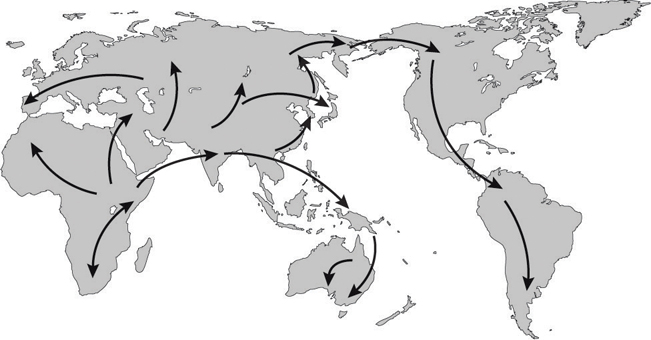
\includegraphics[scale=.40]{Figures/outofafrica.jpg}
		\caption{\scriptsize https://science.education.nih.gov}
	\end{figure}
	
\end{frame}



\begin{frame}
	\frametitle{\bf Population Structure Inference}
	\begin{itemize}
		\item Inference on genetic ancestry differences among individuals from different populations, or {\bf population structure},  has been motivated by a variety of applications: 
		\begin{itemize}
			\item population genetics
			\item  genetic association studies
			\item personalized medicine
			\item forensics 
		\end{itemize}
		\item Advancements in array-based genotyping technologies have largely facilitated the investigation of genetic diversity at remarkably high levels of detail
		\item A variety of methods have been proposed for the identification of genetic ancestry differences among individuals in a sample  using high-density genome-screen data.
	\end{itemize}
\end{frame}




\begin{frame}
	\frametitle{\bf Inferring Population Structure with PCA}
	\begin{itemize}
		\item Principal Components Analysis (PCA) is the most widely used approach for identifying and adjusting for ancestry difference among sample individuals
		\item PCA applied to genotype data can be used to calculate  {\bf principal components} (PCs) that explain differences  among the sample individuals in the genetic data
		\item  The top PCs are viewed as continuous axes of variation that reflect genetic variation due to ancestry in the sample.
		\item Individuals with "similar" values for a particular top principal component will have similar ancestry for that axes.
	\end{itemize}
\end{frame}

\begin{frame}
	\frametitle{\bf Standard Principal Components Analysis (sPCA)}
	\begin{itemize}
		\item sPCA is an unsupervised learning tool for dimension reduction in multivariate analysis.
		\item Widely used in genetics community to infer population structure from genetic data.
		\begin{itemize}
			\item Belief that top principal components (PCs) will reflect population structure in the sample.
		\end{itemize}
		\item Orthogonal linear transformation to a new coordinate system
		\begin{itemize}
			\item sequentially identifies linear
			combinations of genetic markers that explain the
			greatest proportion of variability in the data
			\item these define the axes (PCs) of the new coordinate system
			\item each individual has a value along each PC
		\end{itemize}
		\item EIGENSOFT (Price et al. 2006) is a popular implementation of PCA.
	\end{itemize}
\end{frame}

\begin{frame}
	\frametitle{\bf Data Structure}
	\begin{itemize}
		\item Sample of $n$ individuals, indexed by $i = 1,2,\hdots,n$.
		\item Genome screen data on $m$ genetic autosomal markers, indexed by $l =
		1,2,\hdots,m$.
		\item At each marker, for each individual, we have a genotype value,
		$G_{il}$.
		\begin{itemize}
		\item Here we consider SNP data, so $G_{il}$ takes values 0, 1,
		or 2, corresponding to the number of minor alleles.
	\end{itemize}
		\item We center and standardize these genotype values:
		\begin{eqnarray*}
			z_{il} &=& \frac{G_{il} - 2\hat{p}_l}{\sqrt{2\hat{p}_l(1-\hat{p}_l)}}
		\end{eqnarray*}
		where $\hat{p}_l$ is an estimate of the minor allele frequency for marker $l$.
	\end{itemize}
\end{frame}

\begin{frame}
	\frametitle{\bf Genetic Correlation Estimation}
	\begin{itemize}
		\item Create an $n$ x $m$ matrix, $\mZ$, of centered and standardized genotype
		values, and from this, a $n$ x $n$ genetic correlation matrix (GRM):
		\begin{eqnarray*}
			\widehat\bPsi &=& \frac{1}{m} \mZ \mZ^T
		\end{eqnarray*}
		\item $\widehat\bPsi_{ij}$ is an estimate of the genome wide average genetic
		correlation between individuals $i$ and $j$.
%		\item  sPCA  relies on individuals from the same ancestral population  being more genetically correlated than individuals from different  ancestral populations.
	\item PCA is performed by obtaining the eigendecomposition  $\widehat\bPsi$ 
	\end{itemize}
\end{frame}

\begin{frame}
	\frametitle{\bf Standard Principal Components Analysis (sPCA)}
	\begin{itemize}
		\item  Identify orthogonal axes of variation, i.e. linear combinations of SNPs, that best explain the genotypic variability between the $n$ sample individuals.
		\item The result is: 
		\begin{itemize}
			\item a set of $n$ length $n$ eigenvectors, $(\bV_1, \bV_2,
			\hdots \bV_n)$, where $\bV_d$ is a column vector of coordinates of each individual along axis $d$
			\item each principal component is a different linear combination of the $m$ markers
			\item and a corresponding
			set of $n$ eigenvalues, $(\lambda_1 > \lambda_2 > \hdots > \lambda_n)$, in decerasing order.
			\item The $d^{th}$ principal component (eigenvector) corresponds to eigenvalue $\lambda_d$, where  $\lambda_d$ is proportional to the percentage of variability in the genome-screen data  that is explained by $\bV_{d}$. 
		\end{itemize}
		\item These eigenvectors (PCs) are used as surrogates for population structure 
		
	\end{itemize}
\end{frame}




\begin{frame}
	\frametitle{\bf PCA of Europeans }
\begin{minipage}{.5\textwidth}
	\begin{itemize}
	%		\item  The top principal components are viewed as continuous axes of variation that reflect genetic variation due to ancestry in the sample.
	%		\item Individuals with "similar" values for a particular top principal component will have "similar" ancestry for that axes.
	\item Application of PCA in European samples (Novembre et al., \textit{Nature} 2008)  
	\item Among Europeans for whom all four grandparents originated in the same country, the first two PCs computed using 200k SNPs could map their country of origin quite accurately
\end{itemize}
\end{minipage}% This must go next to `\end{minipage}`
\begin{minipage}{.5\textwidth}
	\begin{figure}
	\centering
	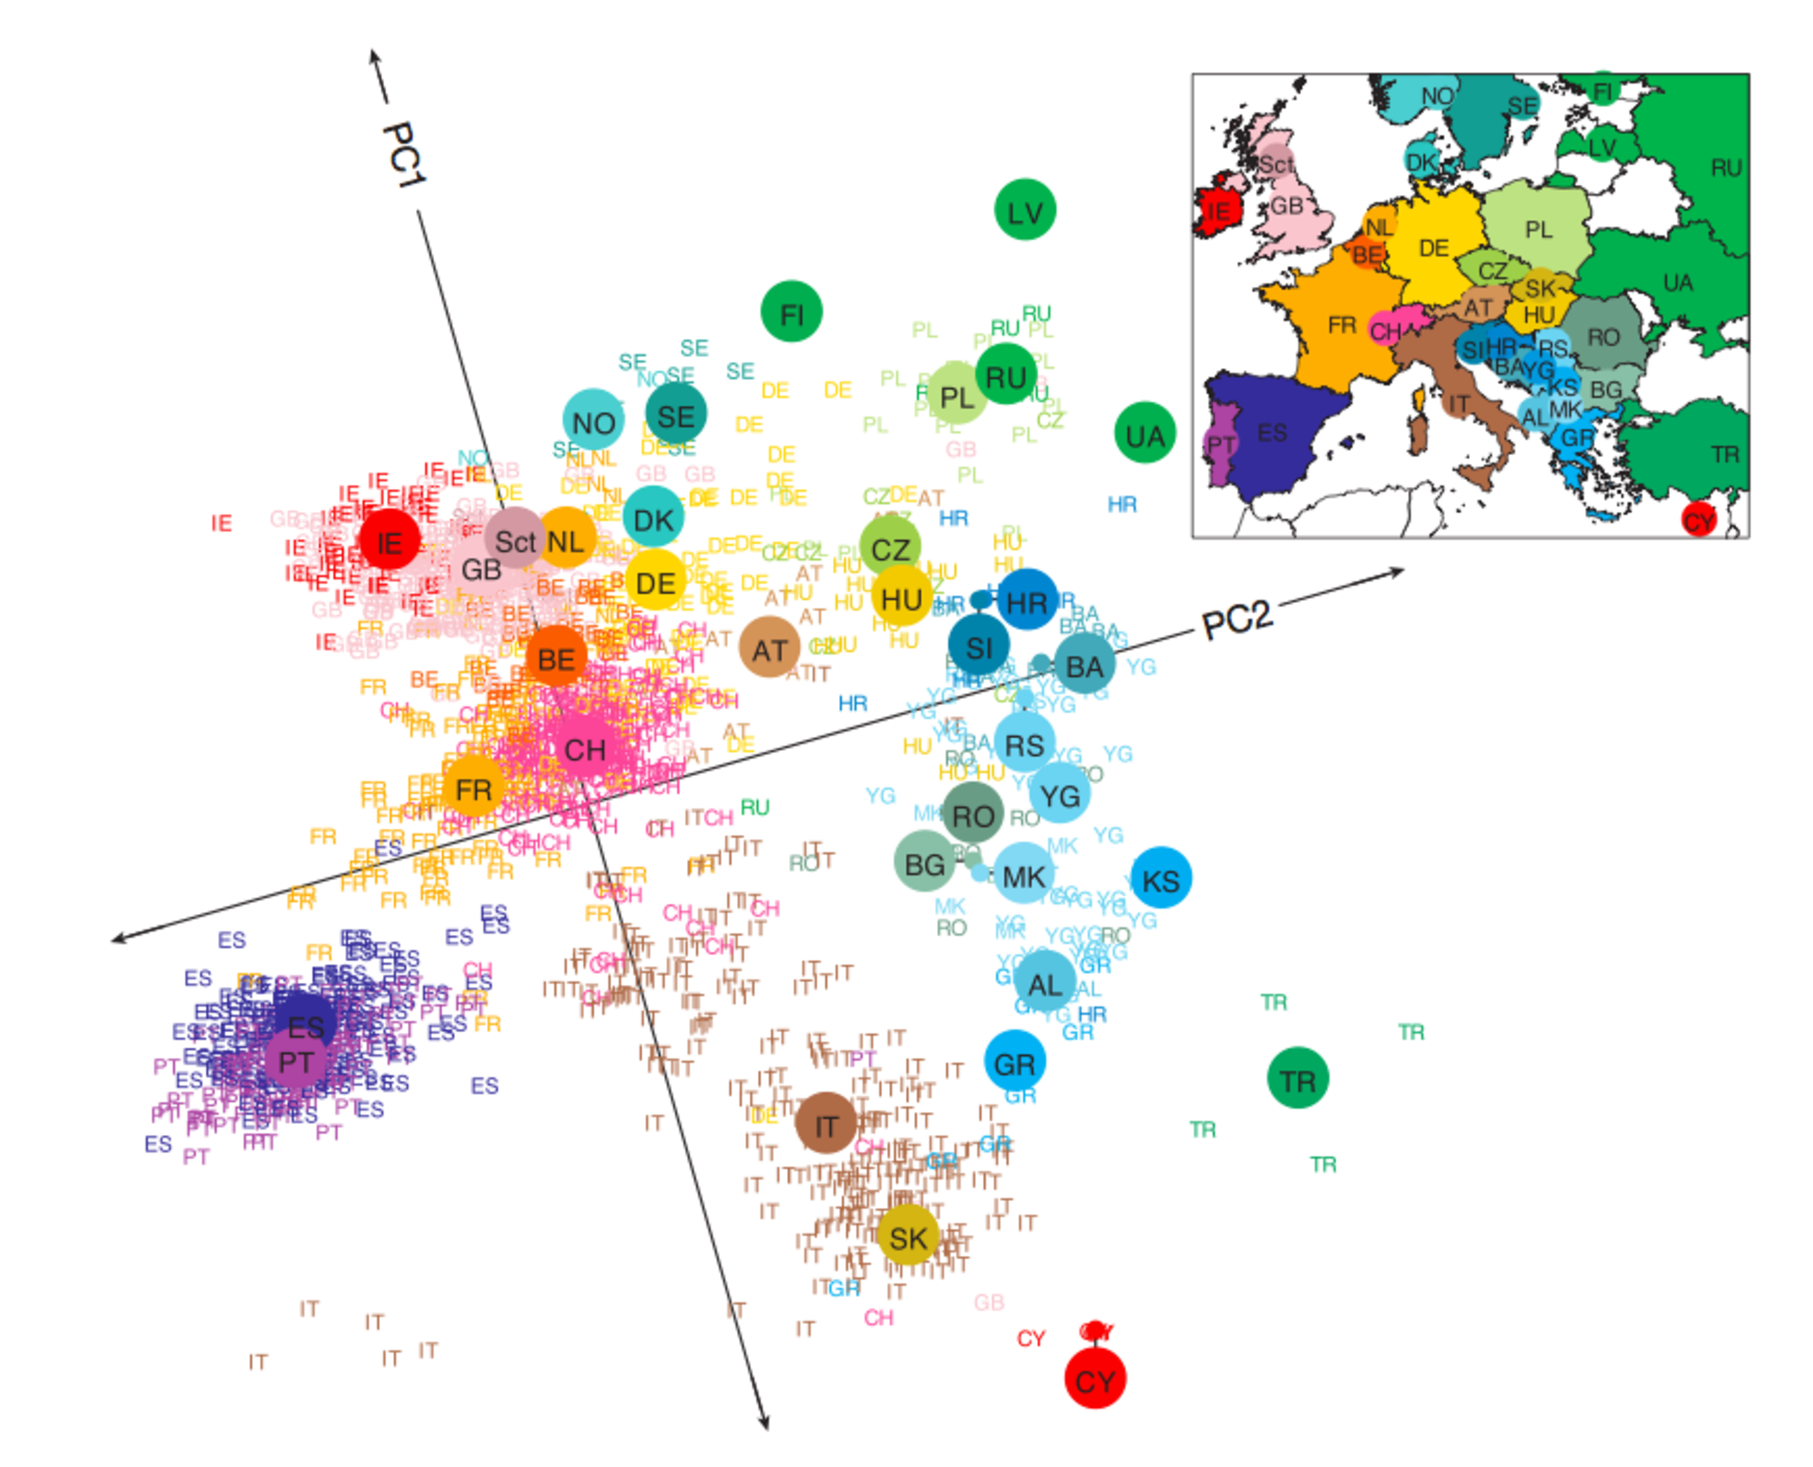
\includegraphics[scale = .2]{Figures/Europe_PCA.pdf}
\end{figure}
\end{minipage}


\end{frame}




\begin{frame}
	\frametitle{\bf Relatedness Confounds sPCA}
	\begin{itemize}
		\item Recall that the GRM used by sPCA, $\widehat\bPsi_{ij}$, and is  an estimate of the genome wide average genetic  correlation between individuals $i$ and $j$.
		\item It can be shown:
		\begin{equation*}
			\bPsi_{ij} = 2\left[\phi_{ij} + (1-\phi_{ij})A_{ij} \right]
		\end{equation*}
		\begin{itemize}
			\item $\phi_{ij}$: kinship coefficient - a measure of familial relatedness
			\item $A_{ij}$:  a measure of ancestral similarity
		\end{itemize}
		\item PCA is an unsupervised method; in related samples we don't know the correlation
		structure each eigenvector is reflecting 
		\begin{itemize}
			\item If the only genetic correlation structure among individuals is due to ancestry, $\bPsi$ and the top PCs will capture this.
			\item If there is relatedness in the sample, the top PCs may reflect this or some combination of ancestry and relatedness.
		\end{itemize}
		\item Association studies have known or cryptic relatedness!
	\end{itemize}
\end{frame}

\begin{frame}
	\frametitle{\bf sPCA: Best practices}
	\begin{itemize}
		\item Apply QC to variants \& samples:
		\begin{itemize}
			\item Restrict to common variants (e.g. MAF $\ge 0.01$)
			\item Remove variants with high missing genotypes rates (e.g. $\geq 0.01$)
		\item Remove variants which fail HWE test (e.g. p-value $\le 10^{-10}$)
		\item Remove samples with high missing genotypes rates (e.g. $\geq 0.1$)
		\item Keep only variants on  autosomal chromosomes
		\end{itemize}
		\item Remove related individuals (e.g. 3rd degree related or closer)
		\item Prune variants in linkage disequilibrium (LD) (e.g. $r^2 \geq 0.2$)
	\end{itemize}
\end{frame}

\section{Population Structure Estimation: bigsnpr}

\begin{frame}[fragile]
	\frametitle{\bf R package bigsnpr}
	\begin{itemize}
			\item   Apply QC to variants \& samples (relies on PLINK2)
	\begin{verbatim} 
snp_plinkQC(plink.path, prefix.in, file.type="--bfile",  
		 maf = 0.01, geno = 0.1, mind = 0.1, hwe = 1e-10,
		 autosome.only = TRUE )
	\end{verbatim}
	\item Remove related individuals (e.g. 3rd degree related or closer)
	\verb| extra.options = "--king-cutoff 0.0442" |
\item Compute PCs
	\begin{itemize}
	\item Prune variants in linkage disequilibrium (LD) (e.g. $r^2 \geq 0.2$)
	\item Removes long-range LD regions
\end{itemize}
\verb| pca <- bed_autoSVD(obj.bed, thr.r2 = 0.2, k = 20)|
\verb| predict(pca)|
\item Project to remaining samples
\verb| bed_projectSelfPCA(object.svd, obj.bed, ind.row)|
	\end{itemize}
\end{frame}


\begin{frame}[fragile]
	\frametitle{\bf R package bigsnpr}
	\vspace{-1em}
		\begin{figure}
		\centering
		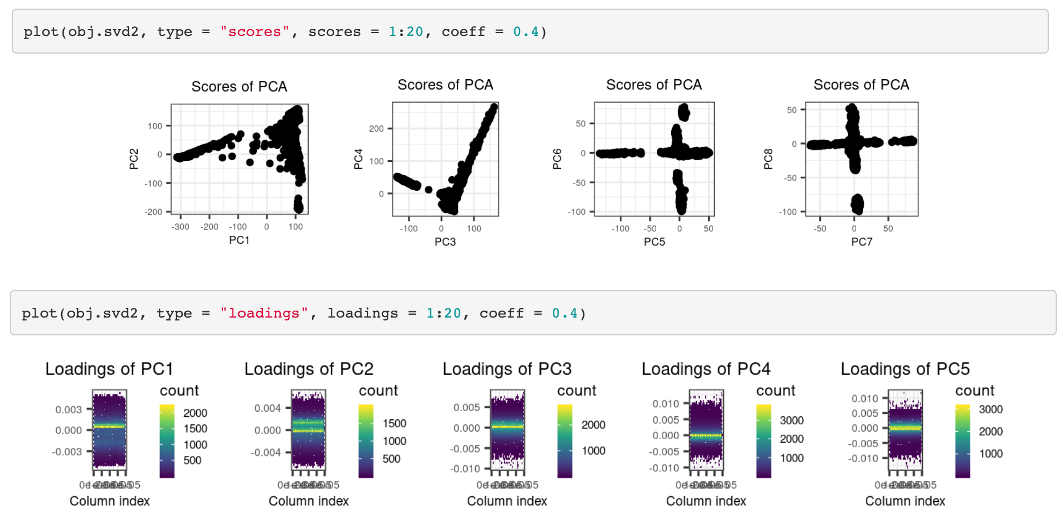
\includegraphics[scale=.40]{Figures/pca_bigsnpr}
		\caption{\scriptsize https://privefl.github.io/bigsnpr/articles/bedpca.html}
	\end{figure}
	

\end{frame}

\section{References}


\begin{frame}
	\frametitle{\bf References}
	\begin{itemize}
		\item Patterson,N., Price, A.L., Reich, D.  (2006) Population structure and eigenanalysis. {\it PLoS Genet.} \textbf{2}, e190.
			\item Novembre, J., Johnson, T., Bryc, K., Kutalik, Z., Boyko, A.R., Auton, A., Indap, A., King, K.S., Bergmann, S., Nelson, M.R. (2008). Genes mirror geography within Europe. {\it Nature}  \textbf{456}, 98-101.
		\item Alexander, D.H., Novembre, J., Lange, K. (2009). Fast model-based estimation of ancestry in unrelated individuals. {\it Genome Res.} \textbf{19},1655-1664.			
	\end{itemize}
\end{frame}



\begin{frame}
	\frametitle{\bf References}
	\begin{itemize}
			\item Conomos MP, Miller M, Thornton T (2015). Robust Inference of Population Structure for Ancestry Prediction and Correction of Stratification in the Presence of Relatedness. {\it Genetic Epidemiology} \textbf{39}, 276-93
		\item Privé, F., Luu, K., Blum, M. G., McGrath, J. J., Vilhjálmsson, B. J. (2020). Efficient toolkit implementing best practices for principal component analysis of population genetic data. \textit{Bioinformatics}, 36(16), 4449-4457.
		\end{itemize}
\end{frame}




\end{document} 






